\documentclass{article}

% ================================= Global settings

\usepackage{amsmath}
\usepackage{amsfonts}
\usepackage[noadjust]{cite}
\usepackage{hyperref}
\usepackage{tikz}
\usepackage{subcaption}
\usepackage{float}
\usepackage[shortlabels]{enumitem}
\usepackage{xcolor} % might not be needed in the end
\usepackage[titlenumbered,ruled]{algorithm2e}

\newtheorem{fact}{Fact}
\newtheorem{lemma}{Lemma}
\newtheorem{theorem}{Theorem}

\DeclareMathOperator{\ps}{ps}

\tikzstyle{hyperedge} = [fill,opacity=.5,fill opacity=.5,line cap=round, line join=round, line width=0pt]

% =================================================

\begin{document}

\section{Introduction}

Propositional satisfiability problem (SAT) is the problem of determining whether a propositional formula in conjunctive normal form (CNF) is satisfiable, i.e. if there exists a truth assignment of variables that satisfies the formula.
Such assignments are called models.
Propositional formulas can be thought of as finite sets of clauses, which in turn are finite sets of literals.
A literal is either a propositional variable or its negation.
Given a CNF formula, a model thus satisfies all its clauses, that is, it sets at least one literal in each clause to true.
Propositional model counting, \#SAT, is a related but harder problem of determining the amount of satisfying truth assignments of a CNF formula.

The complexity class P consists of all problems that can be solved in polynomial time; NP is a class of all problems the solutions of which can be verified in polynomial time. SAT is well known to be NP-complete.
The counting counterpart of NP is the class \#P.
\#SAT has been shown to be \#P-complete and remains \#P-hard even when syntactical restrictions on the input CNF formulas are introduced \cite{DBLP:conf/sat/GanianS17}.
However, there has been research on structural restrictions \cite{DBLP:conf/sat/GanianS17, DBLP:conf/sat/CapelliDM14, DBLP:conf/sat/GanianPSSS22, DBLP:conf/sat/SaetherTV14, DBLP:journals/dam/FischerMR08, DBLP:journals/jda/SamerS10, DBLP:journals/fuin/GanianHO13} which lead to efficient algorithms for \#SAT.

Structural restrictions are defined according to a parameter on some graph associated with the problem instance.
In case of \#SAT, such graphs often describe the relationship between the variables and/or clauses of the formula.
A certain parameter $k$, usually a positive integer, is then determined for this graphic representation of a propositional formula. 
If it's then possible to show that for some fixed $k$, there exists an algorithm that can compute \#SAT in time $f(k)n^{O(1)}$, where $f$ is a computable function and $n$ is the size of the formula, we say that \#SAT is {\em fixed-parameter tractable} when parameterized by $k$ \cite{DBLP:conf/sat/GanianS17}.
As one can see, for a fixed $k$ the term $f(k)$ is a constant, basically meaning that the runtime of the parameterized algorithm is polynomial for such $k$, and such algorithm can therefore be assumed efficient (tractable). The class of fixed parameter tractable problems is denoted FPT.
Its non-parameterized counterpart, FP, is the class of functional problems solvable in polynomial time.

This thesis is organized as follows.
In Section 2, we provide the necessary formal definitions, in particular with regards to graphical representations of formulas, and introduce several structural restrictions, among which are {\em treewidth}, {\em clique-width}, {\em disjoint branches}, {\em twin-width}, {\em rank-width}, {\em ps-width}, and others.



% ---- NEW
\section{Preliminaries}

We first introduce some notions from graph theory which will be useful in this thesis.
We will use these notions to represent propositional formulas, and then perform transformations on them to obtain the desired width parameters.
For examples, see Fig. \ref{fig:graphs}.\\

\begin{figure}
	\centering
	\begin{subfigure}[b]{0.22\textwidth}
		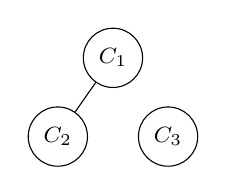
\begin{tikzpicture}[nodes=circle, nodes=draw, font=\footnotesize, minimum size=21pt]
	\node (1) at (0, 0) {$C_1$};
	\node (3) at (-0.7, -1) {$C_2$};
	\node (7) at (0.7, -1) {$C_3$};
	
	\draw (1) to (3);
\end{tikzpicture}

		\caption{}
		\label{fig:consensus}
	\end{subfigure}
	\begin{subfigure}[b]{0.38\textwidth}
		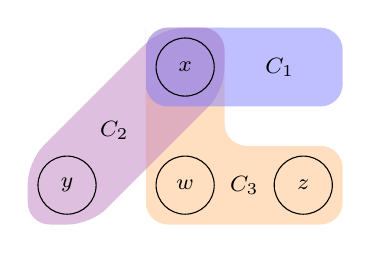
\begin{tikzpicture}[font=\footnotesize, minimum size=21pt]
	\node[circle, draw] (x) at (0, 0) {$x$};
	\node[circle, draw] (y) at (-1.5, -1.5) {$y$};
	\node[circle, draw] (w) at (0, -1.5) {$w$};
	\node[circle, draw] (z) at (1.5, -1.5) {$z$};
	
	\node (c1) at (1.2,0) {$C_1$};
	\node (c2) at (-0.9,-0.8) {$C_2$};
	\node (c3) at (0.75,-1.5) {$C_3$};
	
	\pgfdeclarelayer{background}
	\pgfsetlayers{background,main}
	
	\begin{pgfonlayer}{background}
	\begin{scope}[transparency group,opacity=0.5]
		\fill[hyperedge,color=orange,rounded corners=8pt]
		([shift=({-0.5,0.5})] x.center) -- ([shift=({-0.5,-0.5})] w.center) -- ([shift=({0.5,-0.5})]z.center) -- ([shift=({0.5,0.5})]z.center) -- ([shift=({0.5,0.5})] w.center) -- ([shift=({0.5,0.5})] x.center) -- ([shift=({-0.5,0.5})] x.center) -- ([shift=({-0.5,-0.5})] w.center);
		
		\fill[hyperedge,color=violet,rounded corners=8pt]
		([shift=({0.5,0.5})] x.center) -- ([shift=({-0.3,0.5})] x.center) -- ([shift=({-0.5,0.3})] y.center) -- ([shift=({-0.5,-0.5})] y.center) -- ([shift=({0.3,-0.5})] y.center) -- ([shift=({0.5,-0.3})] x.center) -- ([shift=({0.5,0.5})] x.center) -- ([shift=({-0.3,0.5})] x.center);
		
		\fill[hyperedge,color=blue,rounded corners=8pt]
		([shift=({-0.5,0.5})] x.center) -- ([shift=({-0.5,-0.5})] x.center) -- ([shift=({2,-0.5})] x.center) -- ([shift=({2,0.5})] x.center) -- ([shift=({-0.5,0.5})] x.center) -- ([shift=({-0.5,-0.5})] x.center);
	\end{scope}
	\end{pgfonlayer}
\end{tikzpicture}

		\caption{}
		\label{fig:hypergraph}
	\end{subfigure}
	\begin{subfigure}[b]{0.3\textwidth}
		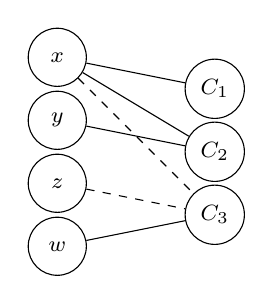
\begin{tikzpicture}[nodes=circle, nodes=draw, font=\footnotesize, minimum size=21pt]
	% consensus
	\node (x) at (0, -0.6) {$x$};
	\node (y) at (0, -1.4) {$y$};
	\node (z) at (0, -2.2) {$z$};
	\node (w) at (0, -3) {$w$};
	
	\node (c1) at (2,-1) {$C_1$};
	\node (c2) at (2,-1.8) {$C_2$};
	\node (c3) at (2,-2.6) {$C_3$};
	
	\draw (x) to (c1);
	\draw (x) to (c2);
	\draw[dashed] (x) to (c3);
	
	\draw (y) to (c2);
	
	\draw[dashed] (z) to (c3);
	\draw (w) to (c3);
\end{tikzpicture}

		\caption{}
		\label{fig:trigraph}
	\end{subfigure}
	\caption{
		Some graphical representations of the formula $C_1 \land C_2 \land C_3$ with $C_1 = \{x\}$, $C_2 = \{x,y\}$ and $C_3=\{\neg x, \neg z, w\}$.
		Here, (a) is the consensus graph, (b) the primal hypergraph, and (c) the signed incidence graph (negative edges are dashed).
		Notice how in (a), $C_3$ does not have any edges, as its literal $\neg x$ appears negated in all other clauses.
	}
	\label{fig:graphs}
\end{figure}

\noindent
\textbf{Graphs}.
A graph is a pair $G = (V,E)$ with a vertex set $V$ and an edge set $E$.
An edge $e=uv$ connects the vertex $u$ to $v$.
A graph is called {\em bipartite} if the vertices can be partitioned into two disjoint sets, and every edge has endpoints in both sets.
There are several commonly known graphs one can define for CNF formulas, such as {\em primal, dual} and {\em incidence graphs}.
In a primal graph, variables of the formula are the graph's vertices, and two vertices are connected by an edge iff both corresponding variables appear together in a clause.
A dual graph's vertices are its clauses, and two vertices are adjacent iff their corresponding clauses share a variable.
An incidence graph is a bipartite graph with variables and clauses both being vertices, and a variable is connected with a clause by an edge iff the variable appears in the clause.
A more recently studied graph is the {\em consensus graph}, where the vertices are the clauses of the formula, and two vertices are connected by an edge iff the clauses do not clash, that is, there exists no literal in one of the clauses that appears negated in the other clause.\\

\noindent
\textbf{Hypergraphs}.
A hypergraph $H=(V,E)$ with vertex set $V$ and (hyper)edge set $E$ is a generalized notion of graphs, where edges may connect not only two, but any amount of vertices.
As such, an edge is a set of vertices it connects.
A CNF formula can be represented by a primal hypergraph, whose vertices are the formula's variables, and hyperedges are the clauses, i.e. hyperedges connect the variables that appear in the clause.\\

\noindent
\textbf{Trigraphs.}
A trigraph $G=(V,E,E')$ is a graph that distinguishes two classes of edges, $E$ and $E'$.
Often such two classes are positive and negative edges, denoted $E^+$ and $E^-$, respectively, in which case the trigraph is called a {\em signed graph}.
A {\em signed trigraph} distinguishes, apart from positive and negative edges, also one more class of edges.
With a CNF formula we associate a signed bipartite incidence graph, where the two classes of vertices are the formula's clauses and variables, and an edge connects a variable with the clause where it appears, with the appropriate sign (according to whether the variable occurs positively or negatively in the clause).

\subsection{Width Parameters}
We now proceed with an introduction of many parameters used to describe the structure of graphs, the so-called {\em width parameters}. \\

\noindent
\textbf{Treewidth} \cite{DBLP:conf/sat/GanianS17}.
For a simple, undirected, finite graph $G = (V,E)$ we define a {\em tree decomposition} to be a pair $(T, B)$, where $T$ is a tree, $B$ a set of {\em bags}, and the vertices of $T$ are the bags.
Each bag is a set of the graph's vertices.
Moreover, a tree decomposition has to fulfil the following two conditions:
\begin{enumerate}
	\item for any edge $uv\in E$ there exists some bag $B' \in B$ such that $\{u,v\} \subseteq B'$, and
	\item for any vertex $v\in V$, $T[\{ b \in B \; | \; v \in b \}]$ is a connected tree with at least one node.
\end{enumerate}
Informally speaking, tree decompositions are a structured way to ``break down'' a graph into its parts.
We define the {\em width} of a tree decomposition to be its maximum bag size minus one, and the {\em treewidth} of $G$, $\textbf{tw}(G)$, to be the minimum width over all its tree decompositions.\\

\noindent 
\textbf{Disjoint branches} \cite{DBLP:conf/sat/CapelliDM14}.
A join tree of a hypergraph $H=(V,E)$ is a pair $(\mathcal{T}, \lambda)$, where $\mathcal{T}=(N,T)$ is a tree with node set $N$ and edge set $T$, and $\lambda : N \rightarrow E$ is a bijection from tree's nodes to hypergraph's edges, which fulfils the following:
\begin{enumerate}
	\item for every $e\in E$, there exists a $t\in N$ such that $\lambda(t)=e$, and
	\item for every $v\in V$, $\mathcal{T}[\{ n \in N \; | \; v \in \lambda(n) \}]$ is a connected subtree of $\mathcal{T}$.
\end{enumerate}
Notice how the definition is similar to that of tree decompositions.
A join tree where for every two nodes $n, n'$ on different branches, $\lambda(n) \cap \lambda(n') = \emptyset$, is called a {\em disjoint branches decomposition}. 
Such decompositions represent a way to ``break down'' a hypergraph into disjoint parts (recall that $\lambda(n)$ is a hypergraph's edge).

We now consider acyclicity of hypergraphs.
In contrast to graphs, there is not just one single but several notions of acyclicity for hypergraphs, such as $\alpha$- (most general), $\beta$- and $\gamma$-acyclicity (least general), all of which can be defined using join trees.

A hypergraph is said to be $\alpha$-acyclic if it has a join tree.
One shortcoming of this definition is that a subhypergraph of an $\alpha$-acyclic hypergraph is not necessarily $\alpha$-acyclic itself.
Thus, a more restrictive notion of $\beta$-acyclicity was introduced, which requires that a hypergraph and all its subhypergraphs be $\alpha$-acyclic.
Admitting a disjoint branches decomposition is itself another notion of hypergraph acyclicity, which lies strictly between $\beta$- and $\gamma$-acyclicity.
As such, having a disjoint branches decomposition implies $\beta$- and $\alpha$-acyclicity.
Finally, a hypergraph is $\gamma$-acyclic if it admits a disjoint branches decomposition for any choice of hyperedge as the root.

Using the four introduced notions of acyclicity, we define the respective classes of hypergraphs, i.e. $\alpha$-, $\beta$-, $\gamma$-acyclic hypergraphs, as well as hypergraphs that admit a disjoint branches decomposition. \\

\noindent
\textbf{Twin-width} \cite{DBLP:conf/sat/GanianPSSS22}.
Consider a trigraph $G=(V,E,R)$ that distinguishes between black ($E$) and red ($R$) edges.
A trigraph whose subgraph induced by the red edges, that is $G[R]$, has maximum degree at most $d$, is called a {\em d-trigraph}.

A {\em contraction} of a trigraph $G$ is a trigraph $G'=G/u,v$ that is a result of contracting two vertices $u,v \in V(G)$ into a single vertex $w$, where the edges of $w$ are determined according to the following:
\begin{itemize}[--]
	\item $wx \in E(G')$ iff $ux, vx \in E(G)$,
	\item $wx \not\in E(G') \cup R(G')$ iff $ux, vx \not\in E(G)\cup R(G),$
	\item $wx \in R(G')$ otherwise.
\end{itemize}
Intuitively, red edges represent ``errors'' that occur during a contraction.
A contraction of a $d$-trigraph is called {\em d-contraction} if it is a $d$-trigraph itself.
If there exists a sequence of $d$-contractions such that a graph is contracted into a single vertex, the graph is called {\em d-collapsible}.
The {\em twin-width} $\textbf{tww}(G)$ of a trigraph $G$ is then the minimal $d$ for which it is $d$-collapsible. \\

% NOTE! signed twin-width. Commented out, if necessary, repeat this in the main part of the thesis.
%
%
%For bipartite trigraphs it is helpful to restrict contraction sequences to those where only vertices from the same partition are contracted.
%That is, for a bipartite trigraph $G$ with $V(G) = A \cup B$, $A \cap B = \emptyset$, there is no contraction of the form $G/a,b$ in the sequence, where $a\in A, b\in B$.
%Such sequences are called {\em bipartite contraction sequences}.
%Notice that no bipartite contraction sequence can end in a single-vertex graph and therefore $d$-collapsibility does not apply.

%We introduce another definition.
%Say a bipartite trigraph $G$ is {\em bipartitely $d$-collapsible} if there exists a sequence of bipartite $d$-contractions such that $G$ is collapsed into a graph with two vertices.
%Then, the {\em signed twin-width} $\textbf{stww}(G)$ of a bipartite trigraph $G$ is the minimal $d$ for which it is bipartitely $d$-collapsible.
%In other words, it is the minimal red degree of all bipartite contraction sequences of $G$.\\

\noindent
\textbf{Clique-width} \cite{DBLP:journals/dam/FischerMR08}.
Colored graphs are graphs with vertices annotated by an integer (color) in $\{1,...,k\}$.
Consider the following set of operations on colored graphs:
\begin{enumerate}
	\item Disjoint union $\oplus$, where $V(A \oplus B)=\{ (v,\, \lambda(v)) \; | \; v \in V(A) \text{ or } v\in V(B) \}$, and $\lambda(v)=$ ``$A$'' if $v\in A$, and $\lambda(v)=$ ``$B$'' if $v\in B$,
	\item Recoloring $\rho_{i,j}(I)$, resulting in a graph where vertices colored $i$ are re-colored $j$,
	\item Edge creation:
	\begin{enumerate}
		\item for unsigned graphs, $\mu_{i,j}(I)$ results in a graph where all vertices colored $i$ are adjacent to all vertices colored $j$,
		\item for signed graphs, $\mu_{i,j}^+(I)$ or $\mu_{i,j}^-(I)$ result in a graph where all vertices colored $i$ are connected to all vertices colored $j$ by a positive or negative edge, respectively. In case of bipartite graphs, vertices from different vertex partitions are not connected.
	\end{enumerate}
\end{enumerate}

\noindent
Notice that the disjoint union is used to introduce single-vertex graphs and avoid name conflicts between vertices.
In particular, $G \oplus G \neq G$.
As an example, consider how one can create cliques using two colors: beginning with two single-vertex graphs $A, B$ colored, say, red (1) and blue (2) respectively, a 2-clique can be obtained as $\mu_{1,2}(A \oplus B)$, a 3-clique as $\mu_{1,2}(\rho_{2,1}(\mu_{1,2}(A \oplus B)) \oplus B)$, and so on.
These expressions (sequence of operations) are called {\em k-expressions} when using at most $k$ colors.
As an example, the 3-clique can be represented as a 2-expression.

{\em Clique-width} $\textbf{cw}(G)$ is defined as the minimal $k$ such that $G$ can be obtained from colored single-vertex graphs using the operations above.
From the example above it is easy to see that cliques have clique-width at most 2.\\

\noindent
\textbf{Branch-width} \cite{DBLP:journals/tocl/LodhaOS19, DBLP:conf/sat/SaetherTV14}.
A branch decomposition of a hypergraph $H$ is a pair $(T, \gamma)$ where $T$ is a binary tree and $\gamma$ is a bijection between the leaves of $T$ and hyperedges of $H$.
For a subset $L$ of leaves, $\gamma(L)$ denotes the set $\{ \gamma(v) \; | \; v \in L \}$, and for a subtree $T'$ of $T$, $\gamma(T')$ is defined as $\{ \gamma(v) \; | \; v  \text{ is a leaf of } T' \}$.

Any subset $E$ of hyperedges of $H$ defines a {\em separation} of $H$, that is the pair $(E,\, E(H) \setminus E)$.
A {\em load vertex} is a vertex that is incident to both an edge in $E$ and an edge in $E(H) \setminus E$.
For a hypergraph $H$ and subset $E$ of hyperedges, $\delta(E)$ is the set of such load vertices of $E$.
In a branch decomposition $(T, \gamma)$ of $H$, any edge $e$ of $T$ similarly defines a separation of the tree. 
We define $\delta(e)$ as the set of load vertices of $\gamma(T')$, that is $\delta(e) = \delta(\gamma(T'))$, where $T'$ is any of the two components in the forest $T \setminus \{e\}$.

The width of an edge $e$ of $T$ is then $|\delta(e)|$, and the width of a branch decomposition is the maximum width over all its edges.
The {\em branch-width} of hypergraph $H$ is the minimum width over all its branch decompositions. In case of $E(H) = \emptyset$, $H$ has no branch decompositions, and its branch-width is said to be 0. \\

\noindent
\textbf{Rank-width} \cite{DBLP:journals/fuin/GanianHO13}.
A set function $f$ maps a subset to a number, i.e. $f : 2^V \rightarrow \mathbb{Z}$, where $V$ is a finite set.
If for all $X,Y \subseteq V$ it holds that $f(X)+f(Y) \geq f(X\cap Y) + f(X\cup Y)$, $f$ is called {\em submodular}.
Moreover, if for all $X\subseteq V$, $f(X) = f(V \setminus X)$, $f$ is said to be {\em symmetric}.

A {\em branch decomposition} of a symmetric, submodular function $f$ is a pair $(T, \lambda)$, where $T$ is a subcubic tree (i.e., every vertex is incident with at most three edges), and $\lambda$ a bijective function from $V$ to the leaves of $T$.
If $\lambda$ is surjective, the branch decomposition is said to be {\em partial}.

For a (partial) branch decomposition $\mathcal{T} = (T,\lambda)$ of $f$ and some edge $e$, $T \setminus e$ is a forest that consists of two connected subtrees of $T$.
Thus $e$ defines a partition $(X,Y)$ of the leaves of the branch decomposition.
The width of the edge $e$ is defined as $f(\lambda^{-1}(X)) = f(\lambda^{-1}(Y))$, and the width of a branch decomposition as the maximum width of all edges of $T$.
Then, the {\em branch-width} of a symmetric, submodular function $f$ is the minimum width over all its branch decompositions.

Consider a simple graph $G$, subsets $X,Y \subseteq V(G)$ and let $\mathbf{A}_G[X,Y]$ be a binary matrix.
The entry $a_{x,y}$ of $\mathbf{A}_G[X,Y]$ is 1 iff $xy \in E(G)$, where $x\in X$, and $y\in Y$.

A {\em cut-rank function} is a symmetric, submodular function $\rho_G : 2^{V(G)} \rightarrow \mathbb{Z}$ such that $\rho_G(X)=\rho_G(V(G)\setminus X) = \text{rank}(\mathbf{A}_G[X, V(G)\setminus X])$.
A {\em rank decomposition} is the branch decomposition of $\rho_G$.
Then, {\em rank-width} $\textbf{rw}(G)$ is the branch-width of $\rho_G$. \\


\noindent
\textbf{ps-width} \cite{DBLP:conf/sat/SaetherTV14}.
ps-width, in contrast to most width parameters introduced above, is defined specifically for propositional formulas.
For a propositional formula $F$, let $\text{var}(F)$ denote the set of variables of $F$, and $\text{cla}(F)$ the set of its clauses.
For a set $C \subseteq \text{cla}(F)$, we say $C$ is {\em precisely satisfiable} in $F$ if there exists some assignment $\tau$ such that $\tau(c)=1$ for all $c\in C$, and $\tau(c)=0$ for all $c \in \text{cla}(F)\setminus C$.
By $\mathcal{PS}(F)$ we denote the set of all sets $C$ such that $C \subseteq \text{cla}(F)$ and $C$ is precisely satisfiable.


A {\em branch decomposition} of a formula $F$ is a pair $(T, \delta)$, where $T$ is a rooted binary tree, and $\delta$ a bijection from the leaves of $T$ to $\text{var}(F) \, \cup \, \text{cla}(F)$.
For an internal (non-leaf) node $v$ of $T$, let $\delta(v) = \{ \delta(l) \; | \; l \text{ is a leaf of subtree rooted in } v \}$.
For any node $v$ of $T$, $\delta(v)$ describes certain cuts of the propositional formula.
Let $F_v$ be then a formula induced by the clauses in cla$(F)\setminus \delta(v)$ and variables in $\delta(v)$, and $F_{\overline{v}}$ a formula induced by the clauses in $\delta(v)$ and the variables in var$(F)\setminus \delta(v)$.

{\em ps-value} ps$(\delta(v))$ of a cut $\delta(v)$ is defined as max$\{|\mathcal{PS}(F_v)|, |\mathcal{PS}(F_{\overline{v}})|\}$, and the {\em ps-width} of a branch decomposition $(T,\delta)$ as max$\{ \text{ps}(\delta(v)) \; | \; v \in V(T) \}$. 
Then, the {\em ps-width} $\mathbf{psw}(F)$ of a formula $F$ is the minimal ps-width over all its branch decompositions.\\

\noindent
\textbf{MIM-width} \cite{DBLP:conf/sat/SaetherTV14, PhD:Vatshelle}.
We once again define {\em branch decompositions}, this time for graphs in general.
A branch decomposition of a graph $G$ is a pair $(T, \delta)$ where $T$ is a rooted binary tree, and $\delta$ a bijection between the leaves of $T$ and $V(G).$
For internal nodes of $T$, $\delta$ is defined in a similar fashion as in branch decompositions of formulas.
A node $n$ analogously defines a cut of the graph, and partitions it, in accordance with $\delta(n)$, into two parts, denoted $(V_n, \overline{V_n})$.

For a graph $G$ and a subset of vertices $V \subseteq V(G)$, a {\em bigraph bipartization} is a bipartite graph $G[V, \overline{V}]$ that is a subgraph of $G$ and that only contains edges with endpoints in both $V$ and $\overline{V} = V(G) \setminus V$.

Consider $G[V_n, \overline{V_n}]$.
An independent set that is also an induced subgraph is called an {\em induced matching}.
We define {\em MIM-value} of a cut $(V_n, \overline{V_n})$ to be the size of the maximum induced matching of $G[V_n, \overline{V_n}]$.
The {\em MIM-width} of a branch decomposition is the maximum MIM-value over all cuts defined by every node.
Then, the {\em MIM-width} $\mathbf{mimw}(G)$ of a graph $G$ is the minimum MIM-width over all branch decompositions of $G$.\\

\noindent
\textbf{Hypertree-width} \cite{DBLP:journals/siamcomp/GottlobP04}.
The {\em hypertree decomposition} of a hypergraph $H=(V,E)$ is defined as the triple $(T, \chi, \lambda)$ where $T$ is a tree, and $\chi, \lambda$ are labelling functions such that  $\chi : V(T) \rightarrow 2^V$ and $\lambda : V(T) \rightarrow 2^E$, where $V(T)$ is the set of vertices (nodes) of $T$.
Apart from that, the following must be fulfilled:
\begin{enumerate}
	\item for every hyperedge $e \in E$, there exists a $v \in V(T)$ s.t. $\{e\} \subseteq \lambda(v)$,
	\item for every vertex $v \in V$, $T[\{ n \in V(T) \; | \; v \in \chi(n) \}]$ is a connected subtree,
	\item for every node $n \in V(T)$, $\chi(n)$ only contains vertices that are incident to at least one hyperedge in $\lambda(n)$, and
	\item for every node $n \in V(T)$, if a vertex $v \in V$ is incident to a hyperedge $e \in \lambda(n)$, and if $v \in \chi(q)$ for some $q$ in a subtree below $n$, then $v\in \chi(n)$.
\end{enumerate}
Then, the {\em width} of a hypertree decomposition is $\max_{n \in V(T)} |\lambda(n)|$, and the {\em hypertree-width} $\mathbf{htw}(H)$ of a hypergraph $H$ is the minimum width over all its hypertree decompositions. \\


\begin{table}
	\centering
	\begin{tabular}{r | c | l}
		\textbf{structural restriction} & \textbf{class} & \textbf{runtime} \\
		\hline
		primal treewidth \cite{DBLP:journals/jda/SamerS10} & FPT  & $\mathcal{O}(2^k(kd+\delta)N)$ \\
		dual treewidth \cite{DBLP:journals/jda/SamerS10} & FPT & $\mathcal{O}(2^k(kl+\delta)N)$ \\
		incidence treewidth \cite{DBLP:journals/jda/SamerS10} & FPT & $\mathcal{O}(2^k(kl+2^k(k+\delta))N)$ \\
		consensus treewidth \cite{DBLP:conf/sat/GanianS17} & FPT  & $2^{\mathcal{O}(k)}\mathcal{O}(L(L+\delta))$ \\
		\hline
		$\alpha$-acyclic hypergraph \cite{DBLP:conf/sat/CapelliDM14} & \#P  & -- \\
		disjoint branches \cite{DBLP:conf/sat/CapelliDM14} & FP & $\mathcal{O}(kr)$ \\
		\hline
		signed incidence clique-width \cite{DBLP:journals/dam/FischerMR08} & FPT & $2^{\mathcal{O}(\text{poly}(k))} \mathcal{O}(n)$ \\
		incidence clique-width \cite{DBLP:conf/isaac/SlivovskyS13} & XP & $\mathcal{O}(m^{6k} l)$ \\
		\hline
		signed incidence twin-width + $k$ \cite{DBLP:conf/sat/GanianPSSS22} & FPT & $d^{\mathcal{O}(kd^2)}\mathcal{O}(n^4)$ \\
		signed incidence rank-width \cite{DBLP:journals/fuin/GanianHO13} & FPT & $\mathcal{O}(2^{3k(k+1)/2}\cdot k^3 n)$ \\
		ps-width \cite{DBLP:conf/sat/SaetherTV14} & FP & $\mathcal{O}(k^3s(m+n))$
	\end{tabular}
	\caption{Complexity results for width parameters on \#SAT instances}
	\label{table:complexity}
\end{table}

\noindent
\textbf{Width parameters for propositional formulas}.
It's possible to introduce structural restrictions on formulas by restricting their graphical representations using the width parameters.
Usually, we are interested in such classes of formulas where the graphical representation is of some bounded width.

For some propositional formula we say that it is of width $k$ if some its graphical representation has width $k$.
We also usually mention which representation is used for determining the width parameter. As such, we refer to {\em primal treewidth}, {\em signed incidence clique-width}, and so on.

Many efficient \#SAT algorithms have been developed for specific classes of formulas with bounded width parameters.
For an overview, refer to Table \ref{table:complexity}.

\subsection{Hierarchy}

Before proceeding to algorithms for \#SAT, we provide a review of the relationships between the width parameters.
Recall that $\mathbf{tw}$, $\mathbf{tww}$, $\mathbf{cw}$, $\mathbf{bw}$, $\mathbf{rw}$, $\mathbf{psw}$, $\mathbf{mimw}$, $\mathbf{htw}$ denote treewidth, twin-width, clique-width, branch-width, rank-width, ps-width, MIM-width, and hypertree-width, respectively.
The following results have been established:
\begin{itemize}[--]
	\item $\mathbf{tww}(G) \leq 2\cdot \mathbf{cw}(G)$ \cite{DBLP:conf/sat/GanianPSSS22},
	\item $\mathbf{cw}(G) \leq 2^{\mathbf{tw}(G)+1}+1$ \cite{DBLP:journals/dam/FischerMR08},
	\item $\mathbf{rw}(G) \leq \mathbf{cw}(G) \leq 2^{\mathbf{rw}(G)+1}-1$ \cite{DBLP:journals/fuin/GanianHO13},
	\item $\mathbf{bw}(G) \leq \mathbf{tw}(G) + 1 \leq \lfloor \frac{3}{2} \, \mathbf{bw}(G) \rfloor$ \cite{DBLP:journals/jct/RobertsonS91},
	\item $\mathbf{rw}(G) \leq \mathbf{bw}(G)$ \cite{DBLP:journals/fuin/GanianHO13},
	\item $\mathbf{mimw}(G) \leq \mathbf{cw}(G)$ \cite{DBLP:conf/sat/SaetherTV14},
	\item $\mathbf{psw}(F) \leq m^{\textbf{mimw}(G_F)}$, for a CNF formula $F$ with $m$ clauses and with incidence graph $G_F$ \cite{DBLP:conf/sat/SaetherTV14},
	\item $\mathbf{htw}(H) \leq \mathbf{cw}(G_H)$, for a hypergraph $H$ with incidence graph $G_H$ \cite{DBLP:journals/siamcomp/GottlobP04}.
\end{itemize}

\noindent
Let \textbf{a} and \textbf{b} be two width parameters.
If there exist computable functions $f,g$ such that $\mathbf{a}(G) \leq f(\mathbf{b}(g(G)))$ for all $G$, parameter \textbf{a} is said to {\em dominate} parameter \textbf{b}å.
Otherwise the two parameters are said to be {\em incomparable}.
With the results above, we establish the domination hierarchy in Fig. \ref{fig:hierarchy}.

\begin{figure}
	\centering
	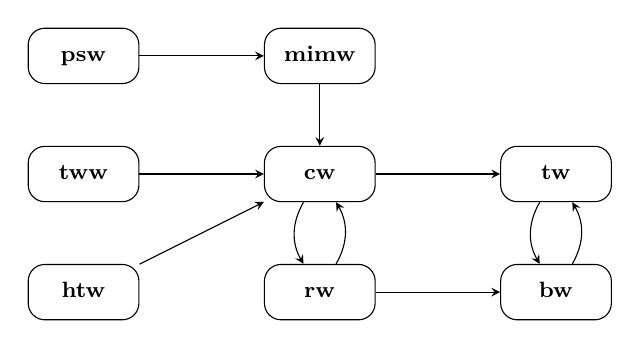
\begin{tikzpicture}[nodes=rectangle, nodes=draw, font=\footnotesize, minimum width=40pt, minimum height=20pt, rounded corners=6pt]
	\node (cw) at (0, 0) {\strut \textbf{cw}};
	\node (tw) at (3, 0) {\strut \textbf{tw}};
	\node (tww) at (-3, 0) {\strut \textbf{tww}};
	\node (rw) at (0, -1.5) {\strut \textbf{rw}};
	\node (bw) at (3, -1.5) {\strut \textbf{bw}};
	\node (mimw) at (0, 1.5) {\strut \textbf{mimw}};
	\node (psw) at (-3, 1.5) {\strut \textbf{psw}}; % strut aligns by baseline
	\node (htw) at (-3, -1.5) {\strut \textbf{htw}};
	
	\draw[-stealth] (psw) to (mimw);
	\draw[-stealth] (mimw) to (cw);
	\draw[-stealth] (tww) to (cw);
	\draw[-stealth] (cw) to (tw);
	\draw[-stealth] (rw) to (bw);
	\draw[-stealth] (htw) to (cw);
	
	\draw[-stealth, bend right] (cw) to (rw);
	\draw[-stealth, bend right] (rw) to (cw);
	
	\draw[-stealth, bend right] (bw) to (tw);
	\draw[-stealth, bend right] (tw) to (bw);
\end{tikzpicture}

	\caption{Domination hierarchy of width parameters. Edges should be read as ``dominates''.}
	\label{fig:hierarchy}
\end{figure}




\section{Graphs of polynomial width}

In this section, we review classes of graphs of bounded width.
In particular, we are interested in such cases where the width parameters are exponentially smaller than theoretically possible, as this would allow to solve \#SAT even more efficiently.

% trees
\textbf{Trees.}
Recall that a tree is a connected graph without cycles.
The following holds:

\begin{fact}[\cite{DBLP:journals/jct/OumS06}]
	If $G$ is a tree, then $\mathbf{tw}(G) = 1$, and $\mathbf{cw}(G) \leq 3$. 
	\label{gw:tree}
\end{fact}

\noindent
The result for treewidth is due to the fact that any tree can be decomposed into bags of size 2.
{\color{lightgray} As there are many ways to construct a graph representation of a CNF formula, we will quickly glance over what effects the restriction of being a tree would have for the corresponding formulas.

Recall that in primal graphs, the vertices are the variables, and the edges connect variables that appear together in a clause.
In a primal tree, each clause of the corresponding formula can be mapped to an edge in the tree.
As such, each clause contains exactly two variables.
Sibling variables (variables corresponding to sibling nodes) never appear together in a clause.

Dual trees correspond to formulas whose clauses are of unbounded size, and two clauses can share any amount of variables. However, for any three clauses it holds $C_1 \cap C_2 \cap C_3 = \emptyset$, as otherwise there would be a cycle.

An incidence graph that is also a tree has the following property: any two vertices at the same depth are either all variables or all clauses, where depth is the distance from some designated root node.
Every clause has exactly $n+1$ variables, where $n$ is the amount of the corresponding node's children.}

% series-parallel
\textbf{Series-parallel graphs.}
Another useful class of graphs of constant treewidth are {\em series-parallel graphs}. The following definitions are inspired by \cite{DBLP:journals/corr/abs-2004-00547}.

A {\em 2-terminal graph} $(G, s, t)$ is a graph $G$ with two designated nodes $s, t$, often called {\em terminals}.
Two 2-terminal graphs $(G_1, s_1, t_1)$, $(G_2, s_2, t_2)$ can be composed as follows:
series-composition results in a 2-terminal graph $(G, s_1, t_2)$, by a disjoint union of the two graphs and then contracting $t_1, s_2$ into one vertex;
and parallel-composition yields a 2-terminal graph $(G, s, t)$, by a disjoint union of the two graphs and then contracting $s_1, s_2$ and $t_1, t_2$ into one vertex each, named $s$ and $t$ respectively.

A 2-terminal graph $(G, s, t)$ is {\em series-parallel} if it is either a two-vertex graph with a single edge,
or it results from a sequence of series- or parallel-compositions of two 2-terminal graphs.
A series-parallel graph is a graph $G$ such that there exist terminals $s, t$ where $(G, s, t)$ is a series-parallel 2-terminal graph.

The following result applies:

\begin{fact}[\cite{DBLP:journals/corr/abs-2004-00547, misc:Hicks04}]
	%\textbf{Fact 2}
	If $G$ is a series-parallel graph, then $\mathbf{tw}(G) = 2$, $\mathbf{bw}(G) \leq 2$. 
\end{fact}

\noindent
We consider graphs of formulas that are isomorphic to series-parallel graphs, i.e. there exists a bijection $\iota : V(G_F) \rightarrow V(G_{\text{sp}})$, where $G_F$ is some graph representation of the formula, and $G_{\text{sp}}$ is a series-parallel graph.

% cliques
\textbf{Complete graphs.}
A complete graph has the property that for any vertex $v$, there exists an edge to every other vertex $u$ in the graph.
A complete graph with $n$ vertices is denoted $K_n$ and is also often called an $n$-clique.
The following holds:
\begin{fact}[\cite{DBLP:conf/focs/Bonnet0TW20, DBLP:journals/dam/FischerMR08}]
	%\textbf{Fact 3} \cite{DBLP:conf/focs/Bonnet0TW20, DBLP:journals/dam/FischerMR08}.
	If $G$ is an $n$-clique, then $\mathbf{tw}(G) = n - 1$, $\mathbf{tww}(G) = 0$, and $\mathbf{cw}(G) = 2$.
\end{fact}

\noindent
The result for treewidth is obvious, since decomposition is only possible into one bag of size $n$.

{\color{lightgray} Primal cliques represent formulas that consist of one clause, and the formula contains $n$ variables if its primal graph is an $n$-clique.
If the dual graph is a clique, it represents the fact that there is a non-empty set of variables that appears in every clause.
For incidence graphs this case is not of much interest, as any $n$-clique for $n > 2$ has a cycle of odd length, which rules out the clique being bipartite; a 2-clique represents a simple formula of one clause containing one variable.}

% grids
\textbf{Path and grid graphs.}
A {\em $d$-dimensional $n$-grid} is a graph $G$ with $V(G) = \{1, 2, ..., n\}^d$, such that two vertices $(x_1, x_2, ..., x_d)$ and $(y_1, y_2, ..., y_d)$ are connected by an edge if and only if $\sum_{i=1}^d |x_i - y_i| = 1$ \cite{DBLP:conf/focs/Bonnet0TW20}.
Common are 1-dimensional grids (known as path graphs or linear graphs) as well as 2-dimensional grids (usual planar grid graphs).

The following holds for path graphs:
\begin{fact}[\cite{DBLP:conf/focs/Bonnet0TW20}]
	%\textbf{Fact 4} \cite{DBLP:conf/focs/Bonnet0TW20}.
	If $G$ is a path with $n$ vertices, then $\mathbf{tw}(G)=1$, and $\mathbf{tww}(G) = 3$.
\end{fact}

\noindent
{\color{lightgray} A primal path represents a formula where every clause has exactly two variables, and there are as many clauses as there are edges in the path.
Any variable appears in the formula exactly two times in different clauses.
A formula represented by a dual path contains clauses that share a set of variables with the adjacent clauses, and for any three clauses it holds that $C_1 \cap C_2 \cap C_3 = \emptyset$.
An incidence path's vertices alternate between variables and clauses, and the represented class of formulas is the same as in primal paths case.
It is easy to see that a primal path can be transformed into an incidence path by inserting clause vertices, and an incidence path into a primal path by removing said clause vertices.}

Since a path graph is a tree, its treewidth is 1 due to Fact \ref{gw:tree}.
The following result is for 2-dimensional grids:
\begin{fact}[\cite{DBLP:conf/focs/Bonnet0TW20, PhD:Vatshelle}]
	%\textbf{Fact 5} \cite{DBLP:conf/focs/Bonnet0TW20, PhD:Vatshelle}.
	If $G$ is an $n \times n$ grid, then $\mathbf{tw}(G) = n$, $\mathbf{tww}(G) = 6$, $\mathbf{cw}(G) = n + 1$, $\mathbf{rw}(G) = n - 1$, and $ \frac{1}{3}n \leq \mathbf{mimw}(G) \leq \frac{1}{2} (n+1)$.
\end{fact}

\noindent
{\color{lightgray} Primal and dual grids tend to represent formulas with many clauses due to their density.
Incidence graphs can also happen to be grids, if the variables and clauses are arranged in a checkerboard pattern.}

% interval graphs
\textbf{Interval graphs.}
An {\em interval graph} is a graph whose intersection model is that of intervals in $\mathbb{R}$ \cite{DBLP:conf/sat/SaetherTV14}.
That is, for some set of intervals in reals, the graph's vertices represent these intervals, and two vertices are connected by an edge if the corresponding intervals intersect.

\begin{fact}[\cite{PhD:Vatshelle}]
	%\textbf{Fact 6} \cite{PhD:Vatshelle}.
	If $G$ is an interval graph with $n$ vertices, then $\mathbf{tw}(G) = n - 1$, $\mathbf{mimw}(G) = 1$, and $\mathbf{cw}(G)$ and $\mathbf{rw}(G)$ are both in $\Theta(\sqrt{n})$.
\end{fact}

\noindent
An {\em interval ordering} of a CNF formula is a linear ordering $\leq $ on variables and clauses of the formula, such that for any variable $x$ and clause $C$: if $x \in C$, then for all variables $y$ s.t. $x \leq y \leq C$ it follows that $y \in C$; and if $C \leq x$, then for all clauses $S$ s.t. $C \leq S \leq x$ it follows that $x \in S$ \cite{DBLP:conf/sat/SaetherTV14}.
A CNF formula has an interval ordering iff its incidence graph is an interval graph \cite{DBLP:conf/sat/SaetherTV14}.

\begin{fact}[\cite{DBLP:conf/sat/SaetherTV14}]
	%\textbf{Fact 7} \cite{DBLP:conf/sat/SaetherTV14}.
	Let $F$ be a CNF formula with $m$ clauses and incidence graph $G_F$.
	If $G_F$ is an interval graph, then $\mathbf{psw}(F) \leq m$.
	\label{fact:psw-interval}
\end{fact}

\noindent
As an example, the formula $F=\{ \{x_1, x_2\}, \{\neg x_2, x_3\} \}$ has an interval ordering $x_1 \leq x_2 \leq C_1 \leq C_2 \leq x_3$, and its incidence graph is an interval graph.

% d-degenerate
\textbf{{\em d}-degenerate graphs.}
A graph is said to be {\em $d$-degenerate} if there exists a linear ordering $\leq$ of vertices such that for any vertex $v$, the amount of neighbors $u$ s.t. $v \leq u$ is at most $d$ \cite{PhD:Vatshelle}.

\begin{fact}[\cite{PhD:Vatshelle}]
	%\textbf{Fact 8} \cite{PhD:Vatshelle}.
	If $G$ is a $d$-degenerate graph with $n$ vertices, then $\mathbf{tw}(G) \leq n - \alpha$, $\mathbf{cw}(G) \leq \frac{2n}{3} - 2\beta - 1$, $\mathbf{rw}(G) \leq \frac{n}{3} - \beta$ and $\mathbf{mimw}(G) \leq \frac{n}{3} - \beta$, where $\alpha = \frac{n}{d + 3} - 2$ and $\beta = \frac{n}{9d+3} - 1$.
\end{fact}

\textbf{Lower bound on complete bipartite graphs.}
A complete bipartite graph $K_{m,n}$ is a bipartite graph with two sets of vertices $U, V$ with $|U|=m, |V|=n$, such that every vertex from $U$ is connected by an edge to every vertex from $V$ (and vice versa).
%$K_{m,n}$ is $\min \{m,n\}$-degenerate and has treewidth $\mathbf{tw}(G) \geq \min \{m,n\}$.

\begin{fact}[folklore]
		It holds that $\mathbf{tw}(K_{m,n}) \geq \min \{m,n\}$, and $\mathbf{cw}(K_{m,n})=2$.
\end{fact}






\section{Utilizing the ps-width of a formula}

\subsection{Computing a branch decomposition}

The algorithm for \#SAT that follows in the next subsection requires a formula and its branch decomposition on input, preferably of as small ps-width as possible.
As no methods for computing branch decompositions with minimal ps-width have been published yet, we opted for an algorithm of Lodha et al. \cite{DBLP:journals/tocl/LodhaOS19}, with the help of which we can minimize the branch-width of the formula's incidence graph.

%Let the depth of a branch decomposition be the radius of its tree.

\begin{theorem}[\cite{DBLP:journals/tocl/LodhaOS19}]
	Given a hypergraph $H$ with $m$ edges and $n$ vertices, we can construct a formula $F(H,w)$ that is satisfiable if and only if $H$ has a branch decomposition of branch-width at most $w$, and that has $\mathcal{O}(m^3 + m^2n^2)$ variables and $\mathcal{O}(m^4n + m^2n^2)$ clauses; and we can construct a branch decomposition from a satisfying assignment in time linear in the number of variables.
\end{theorem}

\noindent
For our purposes, we restrict the edges of the hypergraph $H$ to have a size of exactly two, and as such $H$ degenerates to a graph.
The construction of $F(H,w)$ according to \cite{DBLP:journals/tocl/LodhaOS19} is described next.

In a graph, the {\em eccentricity} of a vertex is the maximum distance between it and any other vertex, and the {\em radius} of a graph is the minimum eccentricity over all vertices.
The {\em depth} of a branch decomposition is the radius of its tree.
We first construct a formula $F(H,w,d)$ that is satisfiable iff $H$ has a branch decomposition of branch-width at most $w$ and depth at most $d$.
Then we choose such $d$ that $F(H,w,d)$ is satisfiable iff $H$ has a branch decomposition of branch-width at most $w$.

Before we proceed, we introduce a way to represent branch decompositions using (weak) partitions.
A {\em weak partition} of a set $S$ is a family $P$ of non-empty, disjoint subsets of $S$.
Let $U(P)$ denote the union of all sets in $P$.
If $S = U(p)$, then $P$ is a (non-weak) partition.
The elements of $P$ are called {\em equivalence classes}.
For two weak partitions $P,P'$, we say $P'$ is a {\em refinement} of $P$ if $U(P) \subseteq U(P')$, and any two elements $x,y \in S$ that are in the same equivalence class of $P$, appear together in one equivalence class of $P'$.
Additionally, if for every $p \in P$ there are $p_1, p_2, ..., p_k$ in $P'$ such that $p \subseteq \bigcup_{1 \leq i \leq k}p_i$, we say $P'$ is a {\em $k$-ary refinement}.
Given a hypergraph $H$, the {\em derivation} of $H$ of length $d$ is a sequence $P_1, P_2, ..., P_d$ of partitions of $E(H)$ such that the following holds:
\begin{enumerate}
	\item $P_1 = \{ \{e\} \, | \, e \in E(H) \}$, and $P_d = \{ E(H) \}$, and
	\item for every $1 \leq i \leq d-2$, $P_i$ is a 2-ary refinement of $P_{i+1}$, and
	\item $P_{d-1}$ is a 3-ary refinement of $P_d$.
\end{enumerate}
The width of a derivation is the maximum size of a set of load vertices $\delta(S)$ in $H$ over all sets $S \in \bigcup_{1\leq i \leq d} P_i$.
We also say $P_i$ is the $i$-th level of the derivation.

\begin{lemma}[\cite{DBLP:journals/tocl/LodhaOS19}]
	Let $H$ be a hypergraph.
	$H$ has a branch decomposition of width at most $w$ and depth at most $d$ if and only if $H$ has a derivation of width at most $w$ and length at most $d$.
\end{lemma}

\noindent
We now describe the construction of $F(H,w,d)$.
We assume the hypergraph $H$ has $m$ edges, $n$ vertices, and its edges and vertices are represented by integers from 1 to $m$ or $n$ respectively.
For two edges $e,f$, we define $e < f$ according to their integer representations.
We introduce the following variables:
\begin{itemize}
	\item[--] {\em set variable} $s(e,f,i)$ is true iff edges $e,f$ are in the same set at level $i$,
	\item[--] {\em leader variable} $l(e,i)$ is true iff $e$ is the smallest edge in some set at level $i$, which is used to identify sets (equivalence classes),
	\item[--] {\em load variable} $c(e,u,i)$ is true iff $u$ is a load vertex of the set containing $e$ at level $i$,
	\item[--] {\em counter variable} $\#(e,u,i,j)$ is true iff $u$ is the lexicographically $j$-th load vertex of the edge $e$ at level $i$.
\end{itemize} 
Then the formula has the following clauses:
\begin{enumerate}
	\item $\neg s(e,f,0) \land s(e,f,d) \land (\neg s(e,f,i) \lor s(e,f,i+1))$,
	 
	for $e,f \in E(H), e<f$, $1 \leq i \leq d$;
	
	\item $\ \ \, (\neg s(e,f,i) \lor \neg s(e,g,i) \lor s(f,g,i))$ \vspace{-4pt}
	
	$\land \, (\neg s(e,f,i) \lor \neg s(f,g,i) \lor s(e,g,i))$ \vspace{-4pt}
	
	$\land \, (\neg s(e,g,i) \lor \neg s(f,g,i) \lor s(e,f,i))$,
	
	for $e,f,g \in E(H), e < f < g$, $1 \leq i \leq d$;
	
	\item $(l(e,i) \lor \bigvee_{f\in E(H), f<e} s(f,e,i)) \land \bigwedge_{f\in E(H), f<e} (\neg l(e,i) \lor \neg s(f,e,i))$,
	
	for $e \in E(H), 1 \leq i \leq d$;
	
	\item $\neg l(e,i) \lor \neg(l,f,i) \lor \neg s(e,f,i+1) \lor l(e,i+1) \lor l(f,i+1)$,
	
	for $e,f \in E(H), e < f, 1 \leq i < d-1$;
	
	\item $\ \ \, \neg l(e,d-1) \lor \neg l(f,d-1) \lor \neg l(g,d-1) \lor \neg s(e,f,d) \lor \neg s(e,g,d)$ \vspace{-4pt}
	
	$\lor\, l(e,d) \lor l(f,d) \lor l(g,d)$,
	
	for $e,f,g \in E(H), e < f < g$;
	
	\item $l(e,i) \lor \neg l(e, i+1)$, for $e \in E(H), 1 \leq i < d$;
	% above were clauses of F(H,d) (in the paper), below the extension to F(H,w,d)
	\item $\neg l(e,i) \lor c(e,u,i) \lor s(\min\{e,f\}, \max\{e,f\}, i) \lor \neg s(\min\{e,g\}, \max\{e,g\}, i)$,
	
	for $e,f,g \in E(H), e\neq f, e\neq g, u \in V(H), u \in f, u \in g, 1 \leq i \leq d$;
	
	\item $\neg l(e,i) \lor s(\min\{e,f\}, \max\{e,f\}, i) \lor c(e,u,i)$,
	
	for $e,f \in E(H), e \neq f, u \in V(H), u \in e, u \in f, 1 \leq i \leq d$;
	
	\item $\neg l(e,i) \lor \neg l(e,i+1) \lor \neg l(e,i+2) \lor \neg c(e,u,i) \lor \neg c(e,u,i+2) \lor c(e,u,i+1)$,
	
	for $e \in E(H), u \in V(H), 1 \leq i \leq d-2$;
	
	\item $(\neg \#(e,u-1,i,j) \lor \#(e,u,i,j)) \land (\neg c(e,u,i) \lor \#(e,u-1,i,j-1) \lor \#(e,u,i,j))$\vspace{-4pt}
	
	$\land \, (\neg c(e,u,i) \lor \neg \#(e,u-1,i,w))$,
	
	for $e \in E(H), 2 \leq u \leq |V(H)|, 1 \leq i \leq d, 1 \leq j \leq w$;
	
	\item $\neg c(e,u,i) \lor \#(e,u,i,1)$, for $e \in E(H), 1 \leq u \leq |V(H)|, 1 \leq i \leq d$.
\end{enumerate}

\noindent
The clauses 1--5 ensure the fulfilment of conditions in the definition of a derivation.
The clauses 6 allow to limit the search space (a non-leader edge at level $i$ cannot become a leader at next levels).
The clauses 7--9 define the load vertices, and the clauses 10--11 restrict the size of sets of load vertices to $w$.
The following lemma lets us fix $d$ to some value, as we are only interested in the width $w$.

\begin{lemma}[\cite{DBLP:journals/tocl/LodhaOS19}]
	Let $H$ be a hypergraph and $e$ the maximum size over all edges of $H$.
	Then the branchwidth of $H$ is at most $w$ if and only if $H$ has a derivation of width at most $w$ and length at most $\lfloor \frac{1}{2} |E(H)| \rfloor - \lceil \frac{w}{e} \rceil + \lceil \log \lfloor \frac{w}{e} \rfloor \rceil$.
\end{lemma}

\noindent
Having obtained a satisfying assignment, we can construct a derivation by looking at the set and leader variables that are set to true.
Then we can transform it into a branch decomposition as follows.
First, we add a leaf for all sets in $P_1$, and then, for every set in $P_2$ that is the union of two sets $S,S'$ in $P_1$, we add an internal node whose children are the nodes corresponding to $S,S'$ (in this case leaves).
This goes on until $P_d$ is reached, where we add a root node whose children are the three nodes corresponding to the sets in $P_{d-1}$.

Although this method allows to compute the exact branch-width, the large amount of variables and clauses in the resulting formula results in large solving times, which would not be practical.
Therefore it is possible to employ a local search algorithm to optimize a branch decomposition obtained by heuristic means.

--------

We propose the diameter method \cite{misc:Hicks04} as a heuristic to obtain a sub-optimal branch decomposition.
A branch decomposition of a graph $G$ is called {\em partial} if its tree contains an internal node with degree larger than three. 
We begin with a partial branch decomposition $(T_1, \gamma)$ where $T_1$ is a star (a tree with $|E(G)|$ leaves, and one internal node $v$ that is adjacent to all the leaves).
One then finds a separation $(A,B)$ of the graph's edges such that $|E(A)|, |E(B)| \geq 2$, and creates a new partial branch decomposition $(T_2, \gamma)$, where $v$ is replaced with two vertices $x$ and $y$, connected by an edge $xy$, and the leaves of $x$ and $y$ correspond to $E(A)$ and $E(B)$, respectively.
A node $a$ with $\deg(a)>3$ is chosen; let $G_a$ be the subgraph of $G$ associated with neighbors of $a$ that are leaves, and $e$ the edge between $a$ and the other internal vertex. \textbf{[unclear - associated? induced?]}
We refer to the load vertices $\delta(e)$ as {\em linking nodes} and find a separation $(X,Y)$ of $G_a$.
Assuming $|X| \leq |Y|$, if $|X|>1$, we create a new partial branch decomposition $(T_3, \gamma)$ with new vertices $x,y$ and edges $ax, ay$, where $x$ has leaves corresponding to $E(X)$ and $y$ leaves corresponding to $E(Y)$.
If $|X|=1$, only one vertex $y$ and the edge $ay$ is created, with leaves of $y$ corresponding to $E(Y)$.
This continues until a (non-partial) branch decomposition is obtained.

The separations are found according to the heuristic.
The {\em diameter} of a graph is the maximum eccentricity over all its vertices.
Assume $(T_i, \gamma)$ is a partial branch decomposition, $a$ an internal node with $\deg(a) > 3$, and $e$ the edge between $a$ and its other internal neighbor.
The separation is chosen as follows.
We label the vertices in $\delta(e)$, as well as vertices with eccentricity equal to the diameter of $G_a$, as {\em source nodes}.
Let $v$ be a source node and $\epsilon$ a real with $0 < \epsilon < 1$.
Sort all nodes according to their distance to $v$ in non-decreasing order, and let $A$ be the set of the first $\lceil \alpha |V(G_a)| \rceil$ and $B$ the set of the last $\lfloor \alpha |V(G_a)| \rfloor$ nodes.

Now we want to compute a separation $(X,Y)$ of $G_a$ such that $A \subseteq V(X),\, B \subseteq V(Y)$ and $|V(X) \cap V(Y)|$ is minimized.
\textbf{[isn't it always 0 as X,Y is a separation?]}
Let $G^-$ be a minor of $G$ with $A$ identified to $v_A$ and $B$ identified to $v_B$.
One then finds sep$(v_A, v_B)$, the smallest vertex cut intersecting all $v_Av_B$-paths.
Label the nodes of sep$(v_A, v_B)$ in $G_a$ as {\em separation nodes}.
In $G_a$, let $sep$ be the amount of separation nodes, $sh$ the amount of nodes that are both linking and separation nodes, $side$ the amount of nodes on one side of the cut but not separation nodes, and $link$ the amount of linking nodes.
Then for a pair $(v, \alpha)$ we can define
\begin{align*}
	work := & \max\{ side + sep,\, link - side - sh + sep \}, \\
	play := & \min\{ side + sep,\, link - side - sh + sep \}.
\end{align*}
Iterate over all source nodes and different values of $\alpha$ and find the pair $(v_o, \alpha_o)$ with the smallest $work$, and the biggest $play$ out of pairs with the same work.

We can use a branch decomposition obtained by this heuristic in the following local improvement algorithm, which has been described in \cite{DBLP:journals/tocl/LodhaOS19}.
Let $H$ be a hypergraph and $B=(T,\gamma)$ its branch decomposition.
For a connected ternary subtree $T_L$ of $T$, the {\em local branch decomposition} is the pair $B_L=(T_l, \gamma_L)$ with $\gamma_L(l) = \delta_B(e)$, where $l$ is a leaf of $T_L$, $e$ the unique edge incident to $l$ in $T_L$, and $\delta_B(e)$ is the set of load vertices of $e$ in $B$.
Moreover, $H(T_L)$ is the hypergraph with a hyperedge $\gamma_L(l)$ for each leaf $l$ of $T_L$, and with vertices that are the union of all these edges.  
The idea behind local improvement is that we can obtain a (possibly more optimal) branch decomposition of $H$ by modifying $B$: in particular by replacing the part formed by $B_L$ with any branch decomposition of $H(T_L)$.
See Algorithms \ref{alg:ps-bd-main}, \ref{alg:ps-bd-localbd}, \ref{alg:ps-bd-improveld} for details.

%local improvement
\begin{algorithm}
	\LinesNumbered
	\caption{Local improvement \cite{DBLP:journals/tocl/LodhaOS19}}
	\label{alg:ps-bd-main}
	
	\SetKwInput{Input}{Input}
	\SetKwInOut{Output}{Output}
	\Input{$H$, a hypergraph}
	\Output{A branch decomposition of $H$}

	$B \gets $ compute a branch decomposition with a heuristic; \tcp{$B = (T, \gamma)$}
	$improved \gets \textsf{true}$\;
	\While{$improved$}{
		$M \gets \text{the set of edges $e$ of $B$ whose $|\delta_B(e)|$ is maximum}$\;
		$C \gets \text{the set of components of $T[M]$}$\;
		$improved \gets \textsf{false}$\;
		\ForEach{$c \in C$}{
			$B_L \gets \mathtt{LocalBD}(B, C)$; \tcp{See Algorithm \ref{alg:ps-bd-localbd}}
			$B'_L \gets \mathtt{ImproveLD}(B_L)$; \tcp{See Algorithm \ref{alg:ps-bd-improveld}}
			\uIf{$B'_L \neq \mathsf{null}$}{
				$B \gets \texttt{Replace}(B, B_L, B'_L)$\;
				$improved \gets \textsf{true}$\;
			}
			\uElse{
				break\;
			}
			\textbf{end}
		}
	}
	\Return $B$\;
\end{algorithm}

\begin{algorithm}
	\LinesNumbered
	\caption{\texttt{LocalBD} \cite{DBLP:journals/tocl/LodhaOS19}}
	\label{alg:ps-bd-localbd}
	
	\SetKwInput{Input}{Input}
	\SetKwInOut{Output}{Output}
	\Input{$B = (T, \gamma)$, a branch decomposition of hypergraph $H$, and a component $C$ of $T$}
	\Output{A local branch decomposition of $B$}

	$w \gets \text{the width of } B$\;
	$T_L \gets C$\;
	\ForEach{$c \in V(H),\, \deg_C(c)=2$}{
		add the unique third neighbor and its edge, incident to $c$, to $T_L$; 
	}
	$Q \gets $ a queue containing the leaves of $T_L$\;
	\While{$Q \neq 0, |T_L| \leq globalbudget-2$}{
		$l \gets Q.$pop()\;
		\If{{\em $l$ is not a leaf of $T$}}{
			$c,c' \gets $ two neighbors of $l$ in $T$ that are not neighbors of $l$ in $T_L$\;
			\If{$\delta_B(\{l,c\}) < w,\, \delta_B(\{l,c'\}) < w$}{
				add $c,c'$ together with their edges, incident to $l$, to $T_L$\;
				$Q$.push($c$)\;
				$Q$.push($c'$)\;
			}
		}
	}
	\Return the local branch decomposition of $B$ represented by $T_L$\;
\end{algorithm}

\begin{algorithm}
	\LinesNumbered
	\caption{\texttt{ImproveLD} \cite{DBLP:journals/tocl/LodhaOS19}}
	\label{alg:ps-bd-improveld}
	
	\SetKwInput{Input}{Input}
	\SetKwInOut{Output}{Output}
	\Input{$B_L = (T_L, \gamma_L)$, a branch decomposition of hypergraph $H(T_L)$}
	\Output{An improved branch decomposition of $H(T_L)$}

	\If{$|T_L| > globalbudget$}{
		\Return \textsf{null}\;
	}
	$w \gets $ the width of $B_L$\;
	\Repeat{$B_D = \mathsf{null}$}{
		$B_D \gets \texttt{SATSolve}(H(T_L), w)$\;
		\If{$B_d \neq \mathsf{null}$}{
			$B'_L \gets B_D$\;
		}
		$w \gets w - 1$\;
	}
	\Return $B'_L$\;
\end{algorithm}











% dynamic algorithm
\subsection{Dynamic algorithm for \#SAT}

Recall that for a CNF formula $F$, var$(F)$ denotes the set of variables and cla$(F)$ the set of clauses of $F$;
similarly by var$(C)$ we denote the corresponding set on clauses.
Moreover, we define lit$(C)$ to be the set of literals in clause $C$.
As an example, for $F = \{ C_1, C_2 \}$ with $C_2 = \{ x_1, \neg x_2 \}$ we have var$(C_2) = \{ x_1, x_2 \}$ and cla$(C_2) = \{ x_1, \neg x_2 \}$.

In this section, we solve \#SAT using an FP algorithm (with the parameter being the ps-width of the formula).

\begin{theorem}
	Given a CNF formula $F$ with $n$ variables and $m$ clauses, of size $s$ and of ps-width $k$, \#SAT can be solved in time $\mathcal{O}(k^3s(m+n))$.
	
	\textbf{Make sure complexity includes computing the branch dcmp!}
\end{theorem}

\noindent
{\em Proof.}
The sketch of the proof is as follows.
First, we show that a branch decomposition of a formula can be computed in polynomial time. TODO!
With that at hand, we present an FP algorithm of S\ae ther, Telle and Vatshelle \cite{DBLP:conf/sat/SaetherTV14} that, given a formula and its branch decomposition, solves \#SAT in polynomial time.

The following steps are as described by S\ae ther, Telle and Vatshelle in \cite{DBLP:conf/sat/SaetherTV14}.
The definition of ps-width relies upon precisely satisfiable sets of a formula, which need to be computed in order for the algorithm to proceed.
Thus:

\begin{lemma}[\cite{DBLP:conf/sat/SaetherTV14}]
	Given a CNF formula $F$ with $n$ variables and $m$ clauses, and a branch decomposition $(T, \delta)$ of ps-width $k$, the sets $\mathcal{PS}(F_v)$ and $\mathcal{PS}(F_{\overline{v}})$, for some $v \in V(T)$, can be computed in time $\mathcal{O}(k^2 \log(k) m(m+n))$.
\end{lemma}

% algorithms for PS-sets
\begin{algorithm}
	\LinesNumbered
	\caption{Computing $\mathcal{PS}(F_v)$ \cite{DBLP:conf/sat/SaetherTV14}}
	\label{alg:ps-f-v}
	
	\SetKwInput{Input}{Input}
	\SetKwInOut{Output}{Output}
	\Input{$\mathcal{PS}(F_{c_1})$ and $\mathcal{PS}(F_{c_2})$, where $c_1, c_2$ are either children of $v$ in $(T, \delta)$}
	\Output{$\mathcal{PS}(F_v)$}

	$L \gets \emptyset$\;
	\ForEach{$(C_1, C_2) \in \mathcal{PS}(F_{c_1}) \times \mathcal{PS}(F_{c_2})$}{
		$C \gets (C_1 \cup C_2) \setminus \text{cla}(\delta(v))$\;
		$L \gets L \cup \{ C \}$\;
	}
	\Return $L$
\end{algorithm}

\begin{algorithm}
	\LinesNumbered
	\caption{Computing $\mathcal{PS}(F_{\overline{v}})$ \cite{DBLP:conf/sat/SaetherTV14}}
	\label{alg:ps-f-negv}
	
	\SetKwInput{Input}{Input}
	\SetKwInOut{Output}{Output}
	\Input{$\mathcal{PS}(F_s)$ and $\mathcal{PS}(F_{\overline{p}})$, where $s$ is the sibling, and $p$ is the parent of $v$ in $(T, \delta)$}
	\Output{$\mathcal{PS}(F_{\overline{v}})$}

	$L \gets \emptyset$\;
	\ForEach{$(C_s, C_p) \in \mathcal{PS}(F_s) \times \mathcal{PS}(F_{\overline{p}})$}{
		$C \gets (C_s \cup C_p) \setminus \text{cla}(\delta(v))$\;
		$L \gets L \cup \{ C \}$\;
	}
	\Return $L$
\end{algorithm}

Computing both sets is identical in procedure and only differs by the inputs.
For $\mathcal{PS}(F_v)$, the precisely satisfiable sets at the children nodes are required; for $\mathcal{PS}(F_{\overline{v}})$, the precisely satisfiable sets of the sibling and the parent node.
This has to do with the fact that both sets can be expressed as follows:
\begin{align*}
	\mathcal{FS}(F_v) &= \{ (C_1 \cup C_2) \cap \text{cla}(F_v) \; | \; C_1 \in \mathcal{PS}(F_{c_1}), C_2 \in \mathcal{PS}(F_{c_2}) \},\\
	\mathcal{FS}(F_{\overline{v}}) &= \{ (C_1 \cup C_2) \cap \text{cla}(F_{\overline{v}}) \; | \; C_1 \in \mathcal{PS}(F_s), C_2 \in \mathcal{PS}(F_{\overline{p}}) \}
\end{align*}

\noindent
for a node $v$ in $(T, \delta)$, where $c_1, c_2$ are children of $v$, and $s, p$ are the sibling and the parent of $v$, respectively.
These recursive relations translate into iterative, dynamic algorithms, refer to Algorithms \ref{alg:ps-f-v} and \ref{alg:ps-f-negv}.
Base cases $\mathcal{PS}(F_l)$ for leaves $l$ and $\mathcal{PS}(F_{\overline{r}})$ for root $r$ can be computed in linear time, as these formulas contain up to one variable.

With a way to compute precisely satisfiable sets of clauses, we can proceed to the main part of the \#SAT algorithm.
For every node $v$ in the branch decomposition, we will compute a table $\mathbf{Tab}_v$ indexed by elements in the product $\mathcal{PS}(F_v) \times \mathcal{PS}(F_{\overline{v}})$.
Each table must fulfil the following constraint:
\begin{equation}
	\mathbf{Tab}_v(C_1, C_2) = |\{ \tau \; | \; \text{sat}(F_v, \tau) = C_1, \, \text{cla}(\delta(v)) \setminus C_2 \subseteq \text{sat}(F, \tau) \}|
	\label{psw:constraint}
\end{equation}
where $C_1 \in \mathcal{PS}(F_v)$, $C_2 \in \mathcal{PS}(F_{\overline{v}})$, $\tau$ is an assignment over var$(\delta(v))$, and sat$(F,\tau) \subseteq \text{cla}(F)$ is a subset of clauses of $F$ such that $\tau$ only satisfies the clauses in this subset and no other clauses.
This constraint ensures that each table stores the partial solutions to the problem.

Let the size of formula $F$ be $s = |\text{cla}(F)| + \sum_{C \in \text{cla}(F)} |\text{lit}(C)|$.

\begin{lemma}[\cite{DBLP:conf/sat/SaetherTV14}]
	Given a CNF formula $F$ of size $s$, as well as a branch decomposition $(T, \delta)$ of ps-width $k$, $\mathbf{Tab}_v$ that satisfies Constraint \ref{psw:constraint} can be computed for an internal node $v \in V(T)$ in time $\mathcal{O}(k^3s)$.
\end{lemma}

The computation of $\mathbf{Tab}_v$ depends on two tables $\mathbf{Tab}_{c_1}$ and $\mathbf{Tab}_{c_2}$ that correspond to the children nodes $c_1, c_2$ of $v$ in the branch decomposition.
See Algorithm \ref{alg:ps-tab-v} for how the computation is performed.
For leaves of the branch decomposition, each entry of $\mathbf{Tab}_l$ is set to either 0, 1, or 2, according to the definition. \textbf{[NOTE:] which def?}

After proceeding on all nodes, the number of satisfying assignments is stored in $\mathbf{Tab}_r(\emptyset, \emptyset)$ at the root $r$ of $(T, \delta)$.

\begin{algorithm}
	\LinesNumbered
	\caption{Computing $\mathbf{Tab}_v$ \cite{DBLP:conf/sat/SaetherTV14}}
	\label{alg:ps-tab-v}
	
	\SetKwInput{Input}{Input}
	\SetKwInOut{Output}{Output}
	\Input{$\mathbf{Tab}_{c_1}$, $\mathbf{Tab}_{c_2}$, where $c_1, c_2$ are children of internal node $v$}
	\Output{$\mathbf{Tab}_v$ that satisfies Constraint \ref{psw:constraint}}

	$\mathbf{Tab}_v : \mathcal{PS}(F_v) \times \mathcal{PS}(F_{\overline{v}}) \gets \{ \{ 0, 0, ... \}, \{ 0, 0, ... \}, ... \}$\; 
	\ForEach{$(C_{c_1}, C_{c_2}, C_{\overline{v}}) \in \mathcal{PS}(F_{c_1}) \times \mathcal{PS}(F_{c_2}) \times \mathcal{PS}(F_{\overline{v}})$}{
		$C_{\overline{c_1}} \gets (C_{c_2} \cup C_{\overline{v}}) \cap \delta(c_1)$\;
		$C_{\overline{c_2}} \gets (C_{c_1} \cup C_{\overline{v}}) \cap \delta(c_2)$\;
		$C_{v} \ \gets (C_{c_1} \cup C_{c_2}) \setminus \delta(v)$\;
		$\mathbf{Tab}_v(C_v, C_{\overline{v}}) \gets \mathbf{Tab}_v(C_v, C_{\overline{v}}) + \mathbf{Tab}_{c_1}(C_{c_1}, C_{\overline{c_1}}) + \mathbf{Tab}_{c_2}(C_{c_2}, C_{\overline{c_2}})$\;
	}
	
	\Return $\mathbf{Tab}_v$
\end{algorithm}

As such we solve \#SAT in time $\mathcal{O}(k^3s(m+n))$, where $n$ is the amount of variables, $m$ the amount of clauses, $s$ the size, and $k$ the ps-width of the branch decomposition of the formula.


% interval graphs
\subsection{Complexity improvements}

The cubic factor $k^3$ in the algorithm utilizing the ps-width of a formula is due to the amount of triples in $\mathcal{PS}(F_{c_1}) \times \mathcal{PS}(F_{c_2}) \times \mathcal{PS}(F_{\overline{v}})$ for every node $v$ with children $c_1, c_2$ \cite{DBLP:conf/sat/SaetherTV14}.
In some cases, it is possible to bring the factor down to $k^2$.

A branch decomposition is called {\em linear} if all its internal nodes induce a path.
In that case, for any node $v$, either $c_1$ or $c_2$ is a leaf, and as such, either $|\mathcal{PS}(F_{c_1})|$ or $|\mathcal{PS}(F_{c_2})|$ is a constant.
The consequence is that $\mathcal{PS}(F_{c_1}) \times \mathcal{PS}(F_{c_2}) \times \mathcal{PS}(F_{\overline{v}})$ has $\mathcal{O}(k^2)$ triples, and the following thus holds:

\begin{theorem}
	Given a CNF formula $F$ with $n$ variables and $m$ clauses, of size $s$ and of ps-width $k$, that admits a linear branch decomposition, \#SAT can be solved in time $\mathcal{O}(k^2s(m+n))$.
	
	\textbf{Make sure complexity includes computing the branch dcmp!}
	\label{theorem:sat-linear-bd}
\end{theorem}

There is a class of formulas for which we can construct a linear branch decomposition, namely formulas with interval orderings, and as such use the results of Theorem \ref{theorem:sat-linear-bd}. 

\begin{theorem}[\cite{DBLP:conf/sat/SaetherTV14}]
	Given a CNF formula $F$ with $n$ variables, $m$ clauses, and of size $s$, it is possible to check whether $F$ has an interval ordering in time $\mathcal{O}(s(m+n))$, and if it does, solve \#SAT in time $\mathcal{O}(m^2s(m+n))$.
\end{theorem}

\noindent
We get the complexity result for \#SAT by combining the results of Theorem \ref{theorem:sat-linear-bd} and Fact \ref{fact:psw-interval}.
We can check whether $F$ has an incidence graph that is an interval bigraph, and as such whether $F$ has an interval ordering, using an algorithm by Rafiey \cite{DBLP:journals/corr/abs-1211-2662}, described next (see also Algorithm \ref{alg:interval-bigraph}).

For a connected bigraph $G$, the {\em pair-digraph} $G^+$ is a directed graph whose vertices are pairs $(u,v) \in V(G),\, u \neq v$.
$G^+$ has edges from $(u,v)$ to $(u',v)$ when $u,v$ are in the same partition of $G$ and $uu' \in E(G),\, vu' \not\in E(G)$; and it also has edges from $(u,v)$ to $(u,v')$ when $u,v$ are in different partitions of $G$ and $vv' \in E(G),\, uv \not\in E(G)$.
For $\alpha, \beta \in V(G^+)$ we also write $\alpha \rightarrow \beta$ if there exists an edge from $\alpha$ to $\beta$.
For a subset $D \subseteq V(G^+)$, a {\em circuit} is a sequence of pairs $(x_0, x_1), (x_1, x_2), ..., (x_n, x_0)$ from $D$.

For a subset $R \subseteq V(G^+)$, the {\em out-section} $N^+[R]$ of $R$ is the set of pairs  $\{ (u, v) \, | \, \exists (u',v') : (u',v') \rightarrow (u,v) \}$.
The {\em envelope} $N^*[R]$ is the smallest set of pairs that contains $R$ and is closed under transitivity and out-section.

For a (strong) component $S$ of $G^+$, the {\em couple component} $S'$ contains swapped pairs, i.e. $S' = \{ (u,v) \, | \, (v,u) \in S \}$.
If $S = S'$, the component $S$ is said to be {\em self-coupled.}
A component is called {\em trivial} if it contains exactly one pair, a {\em source component} if it is trivial and its vertex (pair) has in-degree zero, and a {\em sink component} if it is trivial and its vertex has out-degree zero.

Given a set $R = \{ R_1, R_2, ..., R_k, S \}$ of components of $G^+$ s.t. $N^*[R]$ contains a circuit $C$, and an arbitrary $W \subseteq R \setminus \{S\}$ with $W' = \{ R'_i \, | \, R_i \in W\}$, $S$ is said to be a {\em dictator} for $C$ if $N^*[W' \cup (R \setminus W)]$ also contains a circuit.

The algorithm operates as follows.
Given a bipartite graph $G$, we first compute $G^+$.
If there are any self-coupled components, we can immediately conclude that $G$ is not an interval bigraph.

Otherwise we initialize an empty set $D$ and consider pairs of coupled components $S, S'$.
If $D \cup N^+[S]$ contains no circuits, we add all the pairs in $N^+[S]$ to $D$, and discard $N^+[S']$; otherwise we add the pairs in $N^+[S']$ and discard $N^+[S]$.
If $D$ has a circuit we can again conclude that $G$ is not an interval bigraph, and if we can select exactly one of $S, S'$ in $G^+$, we proceed next.

The algorithm then calculates $N^*[D]$ while filling the set $\mathcal{DT}$ of dictator components.
Then, we create an empty set $D_1$, and for every $S_1 \in \mathcal{DT}$ add the pairs in $N^+[S'_1]$ to $D_1$ [and discard $N^+[S_1]$].
For every $S_2 \in D \setminus \mathcal{DT}$, we add the pairs in $N^+[S_2]$ to $D_1$ [and discard $N^+[S'_2]$].
Finally we set $D=N^*[D_1]$ and check for circuits in $D$.
If they are present, we conclude $G$ is not an interval bigraph.

Otherwise we add the remaining components of $H^+$ outside $D$, into $D$, while adding a sink components $S \subseteq V(H^+) \setminus D$, and discard $S'$.
Finally, we go through the set $D$ and set the ordering $<$ for every pair $(u,v)$ as $u < v$.
Then we can sort through the result and return the interval ordering.

\begin{algorithm}
	\LinesNumbered
	\caption{Recognizing an interval bigraph \cite{DBLP:journals/corr/abs-1211-2662}}
	\label{alg:interval-bigraph}
	
	\SetKwInput{Input}{Input}
	\SetKwInOut{Output}{Output}
	\Input{$G$, a connected bigraph with $V(G) = B \cup W$}
	\Output{An interval ordering of the vertices of $G$, or \textsf{false} if $G$ is not an interval bigraph}
	
	\SetKwFunction{FIntOrdering}{intervalOrdering}
  	\SetKwProg{Fn}{Function}{:}{}
  	\Fn{\FIntOrdering{$G$}}{
        %a\;
        %b\;
        %\KwRet\;
  	%}

	Construct $G^+$; if there are self-coupled components, return \textsf{false}\;
	\tcc{Step 1}
	$D \gets \emptyset$\;
	\ForAll{{\em coupled components $S,S' \subseteq V(G^+)$}}{
		\uIf{{\em no circuit in $D \cup N^+[S]$}}{
			\ForAll{$(x,y) \in N^+[S]$}{
				$D \gets D \cup \{(x,y)\}$, $DCT(x,y) := S$\;
			}
			remove $N^+[S]$ from consideration in this step
		}
		\uElseIf{{\em no circuit in $D \cup N^+[S']$}}{
			\ForAll{$(x,y) \in N^+[S']$}{
				$D \gets D \cup \{(x,y)\}$, $DCT(x,y) := S'$\;
			}
			remove $N^+[S']$ from consideration in this step
		}
		\uElse{\Return \textsf{false}\;}
		\textbf{end}
	}
	
	\tcc{Step 2}
	$E \gets N^*[D], \mathcal{DT} \gets \emptyset$\;
	\While{$\exists (x,y) \in E \setminus D$}{
		$D \gets D \cup \{(x,y)\}, \; E \gets E \setminus \{(x,y)\}$\;
		$DCT(x,y) = \mathtt{dictator}(x,y,D)$\;
		\If{{\em there is a circuit in $D \cup \{(x,y)\}$}}{
			$\mathcal{DT} \gets \mathcal{DT} \cup \{DCT(x,y)\}$
		}
	}
	
	\tcc{Step 3}
	$D_1 \gets \emptyset$\;
	\ForAll{$S \in \mathcal{DT}$}{
		$D_1 \gets D_1 \cup  N^+[S']$\;
	}
	\ForAll{$R \in D \setminus \mathcal{DT}$}{
		$D_1 \gets D_1 \cup  N^+[R] $\;
	}
	$D \gets N^*[D_1]$\;
	\If{{\em there is a circuit in $D$}}{
		\Return \textsf{false}\;
	}
	\tcc{Step 4}
	%\While{{\em $\exists S \not\in D$, $S$ is a sink component}}{
	%	$D \gets D \cup S$\;
	%	??? remove $S'$ from further consideration
	%}
	%\ForAll{$(u,v) \in D$}{set $u < v$\;}
	%
	%\Return $v_1, v_2, ..., v_n$ such that $v_i < v_{i+1}$ for $1 \leq i < n$\;
	}
\end{algorithm}

\begin{algorithm}
	\LinesNumbered
	%\caption{Recognizing an interval bigraph \cite{DBLP:journals/corr/abs-1211-2662}}
	%\label{alg:ps-f-v}
	
	%\SetKwInput{Input}{Input}
	%\SetKwInOut{Output}{Output}
	%\Input{$G$, a connected bigraph with $V(G) = B \cup W$}
	%\Output{An interval ordering of the vertices of $G$, or \textsf{false} if $G$ is not an interval bigraph}
	
	\SetKwBlock{IndentBlock}{\texttt{\hspace{1em} /* Step 4 \hspace{22em} */}}{}
	
  	\IndentBlock{
		%\tcc{Step 4}
		\While{{\em $\exists S \not\in D$, $S$ is a sink component}}{
			$D \gets D \cup S$\;
			remove $S'$ from further consideration
		}
		\ForAll{$(u,v) \in D$}{set $u < v$\;}
		\Return $v_1, v_2, ..., v_n$ such that $v_i < v_{i+1}$ for $1 \leq i < n$\;
	}
	\phantom{}
	\SetKwFunction{FDictator}{dictator}
  	\SetKwProg{Fn}{Function}{:}{}
  	\Fn{\FDictator{$x,y,D$}}{
		\uIf{$(x,y) \in N^+[S]$ {\em for some $S$ in $D$}}{
			\Return $S$\;			
		}
		\uElseIf{{\em $x,y$ from different partitions, $(u,y) \rightarrow (x,y), (u,y) \in D$}}{
			\Return $DCT(u,y)$\;
		}
		\uElseIf{{\em $x,y$ from same partition, $(x,w) \rightarrow (x,y), (x,w) \in D$}}{
			\Return $DCT(x,w)$\;
		}
		\uElseIf{{\em $x,y$ from same partition, $(x,y)$ is by transitivity on $(x,w), (w,y) \in D$}}{
			\Return $DCT(w,y)$\;
		}
		\uElseIf{{\em $x,y$ from different partitions, $(x,y)$ is by transitivity on $(x,w), (w,y) \in D$}}{
			\Return $DCT(x,w)$\;
		}
	}
\end{algorithm}

For a graph $G$ with $|V|$ vertices and $|E|$ edges, the complexity of Algorithm \ref{alg:interval-bigraph} is $\mathcal{O}(|V||E|)$ \cite{DBLP:journals/corr/abs-1211-2662}.
In our case, $G$ is the incidence graph of a formula, and as such $|V|=m+n$ and $|E| = s$, where $m,n,s$ are the amount of clauses, variables, and the size of the formula, respectively.
Thus we can compute the interval ordering for an incidence graph of a formula, provided it exists, in time $\mathcal{O}(s(m+n))$.












% ---------- Bibliography

\bibliographystyle{abbrv}
\bibliography{references}

\end{document}
